\documentclass[12pt,a4paper]{article}
\usepackage{amsmath,amssymb,mathrsfs,tikz,times,pifont}
\usepackage[T1]{fontenc}
\usepackage{enumitem}
\newcommand\circitem[1]{%
\tikz[baseline=(char.base)]{
\node[circle,draw=gray, fill=red!55,
minimum size=1.2em,inner sep=0] (char) {#1};}}
\newcommand\boxitem[1]{%
\tikz[baseline=(char.base)]{
\node[fill=cyan,
minimum size=1.2em,inner sep=0] (char) {#1};}}
\setlist[enumerate,1]{label=\protect\circitem{\arabic*}}
\setlist[enumerate,2]{label=\protect\boxitem{\alph*}}
%%%::::::by chnini ameur :::::::%%%
\everymath{\displaystyle}
\usepackage[left=1cm,right=1cm,top=1cm,bottom=1.7cm]{geometry}
\usepackage[colorlinks=true, linkcolor=blue, urlcolor=blue, citecolor=blue]{hyperref}
\usepackage{array,multirow}
\usepackage[most]{tcolorbox}
\usepackage{varwidth}
\usepackage{float} %pour utiliser l'option [H] qui force l'image à apparaître exactement à l'endroit où elle est placée dans le code.
\tcbuselibrary{skins,hooks}
\usetikzlibrary{patterns}
%%%::::::by chnini ameur :::::::%%%
\newtcolorbox{exa}[2][]{enhanced,breakable,before skip=2mm,after skip=5mm,
colback=yellow!20!white,colframe=black!20!blue,boxrule=0.5mm,
attach boxed title to top left ={xshift=0.6cm,yshift*=1mm-\tcboxedtitleheight},
fonttitle=\bfseries,
title={#2},#1,
% varwidth boxed title*=-3cm,
boxed title style={frame code={
\path[fill=tcbcolback!30!black]
([yshift=-1mm,xshift=-1mm]frame.north west)
arc[start angle=0,end angle=180,radius=1mm]
([yshift=-1mm,xshift=1mm]frame.north east)
arc[start angle=180,end angle=0,radius=1mm];
\path[left color=tcbcolback!60!black,right color = tcbcolback!60!black,
middle color = tcbcolback!80!black]
([xshift=-2mm]frame.north west) -- ([xshift=2mm]frame.north east)
[rounded corners=1mm]-- ([xshift=1mm,yshift=-1mm]frame.north east)
-- (frame.south east) -- (frame.south west)
-- ([xshift=-1mm,yshift=-1mm]frame.north west)
[sharp corners]-- cycle;
},interior engine=empty,
},interior style={top color=yellow!5}}
%%%%%%%%%%%%%%%%%%%%%%%

\usepackage{fancyhdr}
\usepackage{eso-pic}         % Pour ajouter des éléments en arrière-plan
% Commande pour ajouter du texte en arrière-plan
\usepackage{tkz-tab}
\usepackage{pgfplots}

\pgfplotsset{compat=1.18}
\geometry{hmargin=2cm,vmargin=2.5cm}
\AddToShipoutPicture{
    \AtTextCenter{%
        \makebox[0pt]{\rotatebox{80}{\textcolor[gray]{0.7}{\fontsize{5cm}{5cm}\selectfont PGB}}}
    }
}
\usepackage{lastpage}
\fancyhf{}
\pagestyle{fancy}
\renewcommand{\footrulewidth}{1pt}
\renewcommand{\headrulewidth}{0pt}
\renewcommand{\footruleskip}{10pt}
\fancyfoot[R]{
\color{blue}\ding{45}\ \textbf{2026}
}
\fancyfoot[L]{
\color{blue}\ding{45}\ \textbf{Prof:M. BA}
}
\cfoot{\bf
\thepage /
\pageref{LastPage}}
\begin{document}
\renewcommand{\arraystretch}{1.5}
\renewcommand{\arrayrulewidth}{1.2pt}
\begin{tikzpicture}[overlay,remember picture]
\node[draw=blue,line width=1.2pt,fill=purple,text=blue,inner sep=3mm,rounded corners,pattern=dots]at ([yshift=-2.5cm]current page.north) {\begingroup\setlength{\fboxsep}{0pt}\colorbox{white}{\begin{tabular}{|*1{>{\centering \arraybackslash}p{0.28\textwidth}} |*2{>{\centering \arraybackslash}p{0.2\textwidth}|} *1{>{\centering \arraybackslash}p{0.19\textwidth}|} }
\hline
\multicolumn{3}{|c|}{$\diamond$$\diamond$$\diamond$\ \textbf{Lycée de Dindéfélo}\ $\diamond$$\diamond$$\diamond$ }& \textbf{A.S. : 2024/2025} \\ \hline
\textbf{Matière: Mathématiques}& \textbf{Niveau : T}\textbf{S2} &\textbf{Date: 22/05/2026} & \textbf{Durée : 4 heures} \\ \hline
\multicolumn{4}{|c|}{\parbox[c]{10cm}{\begin{center}
\textbf{{\Large\sffamily Composition Du 2$ ^\text{\bf nd} $ Semestre}}
\end{center}}} \\ \hline
\end{tabular}}\endgroup};
\end{tikzpicture}
\vspace{3cm}
 
\section*{\underline{Problème :}\quad\textbf{10 pts}} 

\subsection*{\underline{Partie A:}\quad\textbf{.. pts}}

On donne la fonction $h$ définie sur $]0 ; +\infty[$ par : $h(x) = \ln\left(\dfrac{x+1}{x}\right) - \dfrac{1}{x+1}$

\begin{enumerate}
    \item \textbf{Montrons que $h'(x) = -\dfrac{1}{x(x+1)^2}$}
    
    On a : $h'(x) = \dfrac{x-x-1}{x(x+1)} + \dfrac{1}{(x+1)^2} = \dfrac{-1}{x(x+1)} + \dfrac{1}{(x+1)^2} = \dfrac{-x-1+x}{x(x+1)^2} = -\dfrac{1}{x(x+1)^2}$
    
    Donc \colorbox{green}{$h'(x) = -\dfrac{1}{x(x+1)^2}$} \hfill \textcolor{red}{0,25pt}

    \item \textbf{Dressons le tableau de variation de $h$ sur $]0 ; +\infty[$}
    \begin{itemize}
        \item $\lim\limits_{x \to 0^+} h(x) = \lim\limits_{x \to 0^+} \ln\left(\dfrac{x+1}{x}\right) - \dfrac{1}{x+1}$ \\
        or $\lim\limits_{x \to 0^+} \dfrac{x+1}{x} = +\infty$ donc $\lim\limits_{x \to 0^+} \ln\left(\dfrac{x+1}{x}\right) = +\infty$ et comme $\lim\limits_{x \to 0^+} -\dfrac{1}{x+1} = -1$ alors\\ \colorbox{green}{$\lim\limits_{x \to 0^+} h(x) = +\infty$}
        
        \item $\lim\limits_{x \to +\infty} h(x) = \lim\limits_{x \to +\infty} \ln\left(\dfrac{x+1}{x}\right) - \dfrac{1}{x+1} = \ln(1) + 0 = 0$\\
        \colorbox{green}{$\lim\limits_{x \to +\infty} h(x)=0$}
        \item $h'(x) = -\dfrac{1}{x(x+1)^2} < 0 \ ; \ \forall x > 0$ donc $h$ est strictement décroissante sur $]0 ; +\infty[$.
    \end{itemize}
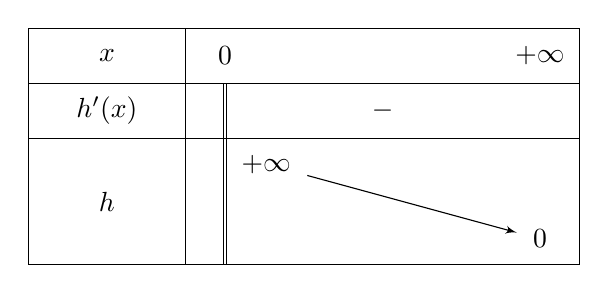
\begin{tikzpicture}
        % On définit l'initialisation du tableau : 
        % espcl=4 augmente l'espace horizontal pour que ce soit plus aéré.
        \tkzTabInit[espcl=4]{$x$ / .7 , $h'(x)$ / .7 , $h$ / 1.6}{$0$, $+\infty$}
        
        % La ligne de la dérivée : 
        % 'd' au début met la double barre en 0, puis on met le signe moins.
        \tkzTabLine{d, -, }
        
        % La ligne des variations de h :
        % D+ / $+\infty$ signifie : au niveau de la double barre (D), la limite est à gauche/haut (+).
        % - / $0$ signifie : la flèche descend (-) vers la valeur 0.
        \tkzTabVar{D+ / $+\infty$, - / $0$}
\end{tikzpicture}

    \hfill \textcolor{red}{0,75pt}

    \item \textbf{Déduisons le signe de $h$ sur $]0 ; +\infty[$.}
    
    D'après le tableau de variation ; on conclut que \colorbox{green}{$h(x) > 0 \ ; \ \forall x > 0$}. \hfill \textcolor{red}{0,25pt}
\end{enumerate}

\newpage

\subsection*{\underline{Partie A:}\quad\textbf{... pts}}

Soit la fonction $f$ définie par $f(x) = \begin{cases} e^{2x} + e^x - 1 & \text{si } x \le 0 \\ 1 - x\ln\left(\dfrac{x}{x+1}\right) & \text{si } x > 0 \end{cases}$ et $(C_f)$ sa courbe représentative dans un repère orthonormé $(O, \vec{i}, \vec{j})$ d'unité $2\text{cm}$.

\begin{enumerate}
    \item \textbf{Montrons que l'ensemble de définition de $f$ est $D_f = \mathbb{R}$.}
    
    Soit $f_1(x) = e^{2x} + e^x - 1$ si $x \le 0$. 
    
    $D_{f_1} = \mathbb{R} \cap ]-\infty ; 0] = ]-\infty ; 0]$
    
    Soit $f_2(x) = 1 - x\ln\left(\dfrac{x}{x+1}\right)$ si $x > 0$. 
    
    $f_2(x)$ existe ssi $\dfrac{x}{x+1} > 0 \ ; \ x + 1 \neq 0$ et $x > 0$
    
    $D_{f_2} = ( ]-\infty ; -1[ \cup ]0 ; +\infty[ ) \cap ]0 ; +\infty[ = ]0 ; +\infty[$.
    
    $D_f = D_{f_1} \cup D_{f_2} = ]-\infty ; 0] \cup ]0 ; +\infty[ = \mathbb{R}$. 
    
    Donc \colorbox{green}{$D_f = \mathbb{R}$} \hfill \textcolor{red}{0,5pt}

    \item \textbf{Calculons $\lim\limits_{x \to -\infty} f(x)$ puis déduisons l'asymptote en $-\infty$.}
    
    $\lim\limits_{x \to -\infty} f(x) = \lim\limits_{x \to -\infty} e^{2x} + e^x - 1 = 0 + 0 - 1 = -1$.
    
     \colorbox{green}{$\lim\limits_{x \to -\infty} f(x) = -1$} \hfill \textcolor{red}{0,25pt}
    
    On a une \colorbox{green}{asymptote horizontale d'équation $y = -1$ en $-\infty$} \hfill \textcolor{red}{0,25pt}

    \item \textbf{Vérifions que si $x > 0$ alors $f(x) = 1 + \dfrac{\ln\left(\frac{x}{x+1}\right)}{\frac{x+1}{x}-1}\left(\dfrac{x}{x+1}\right)$. Déduisons $\lim\limits_{x \to +\infty} f(x)$ puis précisons l'asymptote en $+\infty$.}
    
    \begin{itemize}
        \item .\\
     		$\begin{aligned}
     		1 + \dfrac{\ln\left(\frac{x}{x+1}\right)}{\frac{x+1}{x}-1}\left(\dfrac{x}{x+1}\right) &= 1 + \dfrac{\ln\left(\frac{x}{x+1}\right)}{\frac{1}{x+1}}\left(\dfrac{x}{x+1}\right) \\
     		&= 1 - \ln\left(\dfrac{x}{x+1}\right)(x+1)\left(\dfrac{x}{x+1}\right) \\
     		&= 1 - x\ln\left(\dfrac{x}{x+1}\right)
        \end{aligned}$   		   
         \hfill \textcolor{red}{0,25pt}
        
        \item $
        \begin{aligned}
        \lim\limits_{x \to +\infty} f(x) &= \lim\limits_{x \to +\infty} 1 + \dfrac{\ln\left(\frac{x}{x+1}\right)}{\frac{x}{x+1}-1}\left(\dfrac{x}{x+1}\right)\\ 
        &= 1 + 1 \times 1 \\
        &= 2
        \end{aligned}$ 
        
        Donc \colorbox{green}{$\lim\limits_{x \to +\infty} f(x) = 2$} \hfill \textcolor{red}{0,25pt}
        
        \item On a une \colorbox{green}{asymptote horizontale d'équation $y = 2$ en $+\infty$} \hfill \textcolor{red}{0,25pt}
    \end{itemize}

    \item \textbf{Étudions la continuité et la dérivabilité de $f$ en 0. Interpréter les résultats.}
    \begin{itemize}
        \item \underline{Continuité en 0}
        
        $f(0) = e^0 + e^0 - 1 = 1$
        
        $
        \begin{aligned}
        \lim\limits_{x \to 0^-} f(x) &= \lim\limits_{x \to 0^-} e^{2x} + e^x - 1\\ 
        &= 1
        \end{aligned}$
        
        $
        \begin{aligned}
        \lim\limits_{x \to 0^+} f(x) &= \lim\limits_{x \to 0^+} 1 - x\ln\left(\dfrac{x}{x+1}\right) \\
        &= \lim\limits_{x \to 0^+} 1 - x\ln x + x\ln(x+1)\\ 
        &= 1 - 0 + 0\\
        & = 1
        \end{aligned}$
        
        \colorbox{green}{$\lim\limits_{x \to 0^-} f(x) = \lim\limits_{x \to 0^+} f(x) = f(0)$ donc $f$ est continue en 0.} \hfill \textcolor{red}{0,5pt}
        
        \item \underline{Dérivabilité en 0}
        
        $
        \begin{aligned}
        \lim\limits_{x \to 0^-} \dfrac{f(x)-f(0)}{x-0} &= \lim\limits_{x \to 0^-} \dfrac{e^{2x}+e^x-1-1}{x}\\ 
        &= \lim\limits_{x \to 0^-} \dfrac{e^{2x}-1}{x} + \dfrac{e^x-1}{x}\\ 
        &= 2 + 1 \\
        &= 3
        \end{aligned}
        $
        
        Donc {\color{blue}$f'_g(0) = 3$}
        
        $
        \begin{aligned}
				\lim\limits_{x \to 0^+} \dfrac{f(x)-f(0)}{x-0} &= \lim\limits_{x \to 0^+} \dfrac{1-x\ln\left(\frac{x}       				{x+1}\right)-1}{x}\\ 
				&= \lim\limits_{x \to 0^+} -\ln\left(\dfrac{x}{x+1}\right)\\
				&= +\infty
				 \end{aligned}
        $

        Donc {\color{blue}$\lim\limits_{x \to 0^+} \dfrac{f(x)-f(0)}{x-0} = +\infty$}
        
        $f$ est dérivable à gauche de 0 mais pas dérivable à droite de 0. On conclut que :
        
         \colorbox{green}{$f$ n'est pas} \colorbox{green}{dérivable en 0.} \hfill \textcolor{red}{0,5pt}
        
        \item \underline{Interprétation}
        \begin{itemize}
            \item[$\succ$] À gauche de 0 ; on a \colorbox{green}{une demi-tangente d'équation $(T_g) : y = 3x + 1$} \hfill \textcolor{red}{0,25pt}
            \item[$\succ$] À droite de 0 ; on a \colorbox{green}{une demi-tangente verticale dirigée vers le haut.} \hfill \textcolor{red}{0,25pt}
        \end{itemize}
    \end{itemize}

    \item \textbf{Donnons $f'(x)$ si $x \le 0$ puis montrons que si $x > 0$ ; $f'(x) = h(x)$.}
    
    si $x \le 0$ ; $f$ est dérivable et on a : 
    
    \colorbox{green}{$f'(x) = 2e^{2x} + e^x$} \hfill \textcolor{red}{0,25pt}
    
    si $x > 0$ ; $f$ est dérivable et on a : 
    
    $
     \begin{aligned}
        f'(x) &= -\ln\left(\dfrac{x}{x+1}\right) - \dfrac{1}{x+1}\\
         &= \ln\left(\dfrac{x+1}{x}\right) - \dfrac{1}{x+1}\\ 
         &= h(x)
      \end{aligned}
     $
    
    D'où \colorbox{green}{$f'(x) = h(x)$} \hfill \textcolor{red}{0,5pt}

    \item \textbf{Étudions les signes de $f'$ puis dresser le tableau de variation de $f$ sur $D_f$.}
    \begin{itemize}
        \item si $x \le 0$ ; $f'(x) = 2e^{2x} + e^x > 0$ \hfill \textcolor{red}{0,25pt}
        \item si $x > 0$ ; $f'(x) = h(x) > 0$ \hfill \textcolor{red}{0,25pt}
    \end{itemize}

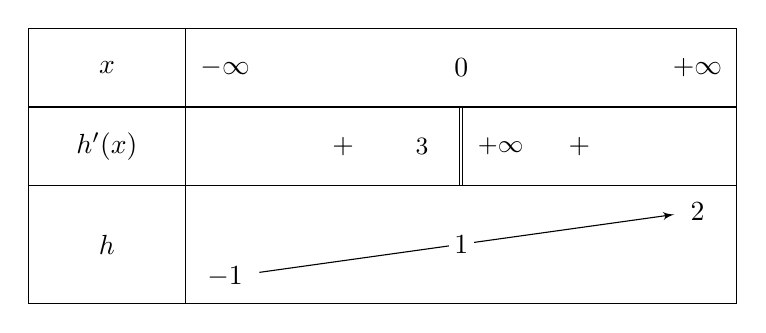
\begin{tikzpicture}
   \tkzTabInit{$x$ /1, $h'(x)$ /1, $h$ /1.5} {$-\infty$ , $0$, $+\infty$}
   \tkzTabLine{, +, d, +, } 
   \tkzTabVar{-/$-1$, R/, +/ $2$}
   \tkzTabIma{1}{3}{2}{$1$}
   \node at (5,-1.5) {\small $3$};
   \node at (6,-1.5) {\small $+\infty$};
\end{tikzpicture}

    \hfill \textcolor{red}{0,75pt}

    \item \textbf{Montrons que l'équation $f(x) = 0$ admet une unique solution $\alpha$ sur $]-\infty ; 0]$ puis vérifier que }
    
    \colorbox{green}{$-0,5 \le \alpha \le -0,4$}
    
    $f$ est bijective de $]-\infty ; 0]$ vers $]-1 ; 1]$ et $0 \in ]-1 ; 1]$ donc 
    
    \colorbox{green}{$f(x) = 0$ admet une unique solution $\alpha$} \colorbox{green}{sur $]-\infty ; 0]$} \hfill \textcolor{red}{0,25pt}
    
    $f(-0,5) \times f(-0,4) \approx -0,003 < 0$ donc \colorbox{green}{$-0,5 \le \alpha \le -0,4$} \hfill \textcolor{red}{0,25pt}

    \item \textbf{Soit $g$ ; la restriction de $f$ sur $I = ]-\infty ; 0]$.}
    \begin{enumerate}
        \item \textbf{Montrons que $g$ est bijective de $I$ vers $J$ à préciser.}
        
        $g$ est continue et strictement croissante sur $I = ]-\infty ; 0]$ donc $g$ est bijective de $I$ vers \colorbox{green}{$J = g(I) = ]-1 ; 1]$} \hfill \textcolor{red}{0,25pt}
        
        \item \textbf{Calculons $g(-\ln 2)$ puis $(g^{-1})'\left(-\dfrac{1}{4}\right)$. Quelle est alors la position relative de la tangente à la courbe $(C_{g^{-1}})$ au point d'abscisse $-\dfrac{1}{4}$ par rapport la première bissectrice ?}
        \begin{itemize}
            \item $g(-\ln 2) = e^{2(-\ln 2)} + e^{-\ln 2} - 1 = \dfrac{1}{4} + \dfrac{1}{2} - 1 = -\dfrac{1}{4}$ \\
            \colorbox{green}{$g(-\ln 2) = -\dfrac{1}{4}$} \hfill \textcolor{red}{0,25pt}
            
            \item $(g^{-1})'\left(-\dfrac{1}{4}\right) = \dfrac{1}{g'(-\ln 2)}$ or $g'(-\ln 2) = 2e^{2(-\ln 2)} + e^{-\ln 2} = \dfrac{2}{4} + \dfrac{1}{2} = 1$ donc \colorbox{green}{$(g^{-1})'\left(-\dfrac{1}{4}\right) = 1$} \hfill \textcolor{red}{0,5pt}
            
            \item \colorbox{green}{La tangente à la courbe $(C_{g^{-1}})$ au point d'abscisse $-\dfrac{1}{4}$ est parallèle à la première} 
            
            \colorbox{green}{bissectrice puisqu'elles ont le même coefficient directeur 1.} \hfill \textcolor{red}{0,25pt}
        \end{itemize}
        
        \item \textbf{Dressons le tableau de variation de $g^{-1}$ sur $J$.}
        
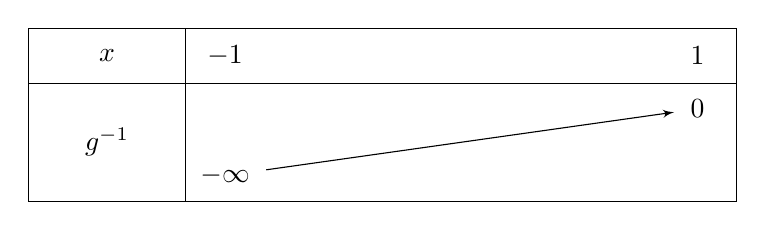
\begin{tikzpicture}
        % Initialisation du tableau pour g^(-1) sur l'intervalle J = ]-1 ; 1]
        % On définit la hauteur des lignes pour correspondre à l'image
        \tkzTabInit[espcl=6]{$x$ / .7 , $g^{-1}$ / 1.5}{$-1$, $1$}
        
        % Ligne des variations de la fonction g^(-1) :
        % La fonction croît de -\infty (en bas à gauche) vers 0 (en haut à droite)
        \tkzTabVar{ - / $-\infty$ , + / $0$ }
\end{tikzpicture}
        \hfill \textcolor{red}{0,25pt}
    \end{enumerate}

    \item \textbf{Traçons les courbes $(C_f)$ et $(C_{g^{-1}})$ dans le même repère.}
    
    \textit{(Se référer au graphique fourni dans les documents originaux contenant $(\mathcal{E}_f)$, $(\mathcal{E}_{g^{-1}})$, la droite $y=x$, ainsi que les asymptotes $y=-1$ et $y=2$.)} \hfill \textcolor{red}{1pt+0,5pt}

\begin{center}
    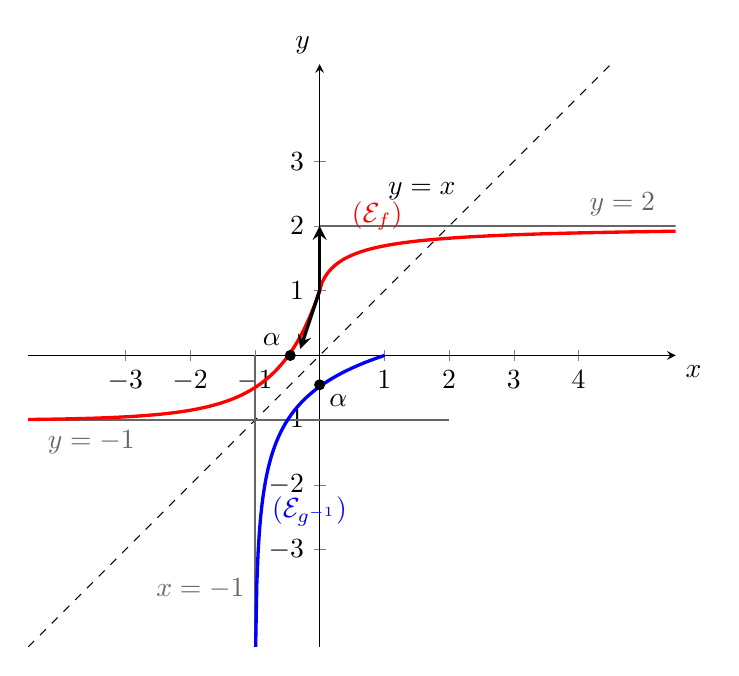
\begin{tikzpicture}
        \begin{axis}[
            axis lines=middle,
            xlabel={$x$}, ylabel={$y$},
            xmin=-4.5, xmax=5.5,
            ymin=-4.5, ymax=4.5,
            xtick={-3,-2,-1,1,2,3,4},
            ytick={-3,-2,-1,1,2,3},
            unit vector ratio=1 1,
            grid=none,
            scale=1.3,
            every axis x label/.style={at={(current axis.right of origin)},anchor=north west},
            every axis y label/.style={at={(current axis.above origin)},anchor=south east}
        ]
            % Première bissectrice y = x
            \addplot[dashed, domain=-4.5:4.5, samples=2] {x} node[pos=0.75, above left] {$y=x$};
            
            % Asymptotes horizontales et verticales
            \addplot[thick, color=black!60, domain=-4.5:2] {-1} node[pos=0.15, below] {$y=-1$};
            \addplot[thick, color=black!60, domain=0:5.5] {2} node[pos=0.85, above] {$y=2$};
            \draw[thick, color=black!60] (axis cs:-1,-4.5) -- (axis cs:-1,0) node[pos=0.2, left] {$x=-1$};
            
            % Courbe (Cf) pour x <= 0
            \addplot[red, very thick, domain=-4.5:0, samples=100] {exp(2*x) + exp(x) - 1};
            % Courbe (Cf) pour x > 0
            \addplot[red, very thick, domain=0.001:5.5, samples=150] {1 - x*ln(x/(x+1))} node[pos=0.3, above left] {$(\mathcal{E}_f)$};
            
            % Courbe (C_g^-1) réciproque sur J = ]-1, 1]
            % Trouvé par inversion x = exp(2y) + exp(y) - 1 => exp(y) = (-1 + sqrt(5+4x))/2
            \addplot[blue, very thick, domain=-0.99:1, samples=100] {ln((-1 + sqrt(5 + 4*x))/2)} node[pos=0.4, right] {$(\mathcal{E}_{g^{-1}})$};
            
            % Tangentes et points remarquables (Alpha)
            \node[above left] at (axis cs:-0.45, 0) {$\alpha$};
            \node[below right] at (axis cs:0, -0.45) {$\alpha$};
            \fill (axis cs:-0.453, 0) circle (2pt);
            \fill (axis cs:0, -0.453) circle (2pt);
            
            % Demi-tangentes en (0,1)
            \draw[->, >=stealth, very thick] (axis cs:0,1) -- (axis cs:-0.3,0.1);
            \draw[->, >=stealth, very thick] (axis cs:0,1) -- (axis cs:0,2);
        \end{axis}
    \end{tikzpicture}
    \end{center}
\end{enumerate}    
   

\end{document}
